\documentclass{article}
\usepackage{graphicx}
\usepackage{hyperref}
\usepackage[margin=1in]{geometry}

\title{Market Basket Analysis on Amazon Book Reviews}
\author{Your Name(s)}
\date{Academic Year 2024/2025}

\begin{document}
\maketitle

\section{Dataset Description}
We used the \textbf{Amazon Books Review} dataset published on Kaggle. The dataset contains:
\begin{itemize}
    \item \texttt{Books\_rating.csv} – includes reviews with fields like \texttt{review/text}.
    \item \texttt{books\_data.csv} – includes metadata like \texttt{User\_id}, \texttt{Title}, and ratings.
\end{itemize}

For our analysis:
\begin{itemize}
    \item For word-based baskets: we used the \texttt{review/text} column.
    \item For book-based baskets: we used \texttt{User\_id} and \texttt{Title}.
\end{itemize}

\section{Data Preprocessing}
\subsection*{Text Reviews}
\begin{itemize}
    \item Dropped duplicates and missing reviews.
    \item Filtered reviews to keep only those with 10–100 words.
    \item Cleaned the text: lowercased, removed punctuation, stopwords, and kept only common words.
\end{itemize}

\subsection*{Book-User Data}
\begin{itemize}
    \item Selected only \texttt{User\_id} and \texttt{Title}.
    \item Filtered out users with only one book reviewed.
    \item Grouped book baskets by user.
\end{itemize}

\section{Methodology}
We used the \texttt{mlxtend} Python library to apply the Apriori algorithm:
\begin{itemize}
    \item Minimum support: 0.01
    \item Minimum confidence: 0.3
\end{itemize}

\section{Experimental Results}
\subsection*{Top Frequent Word Pairs}
\begin{center}
    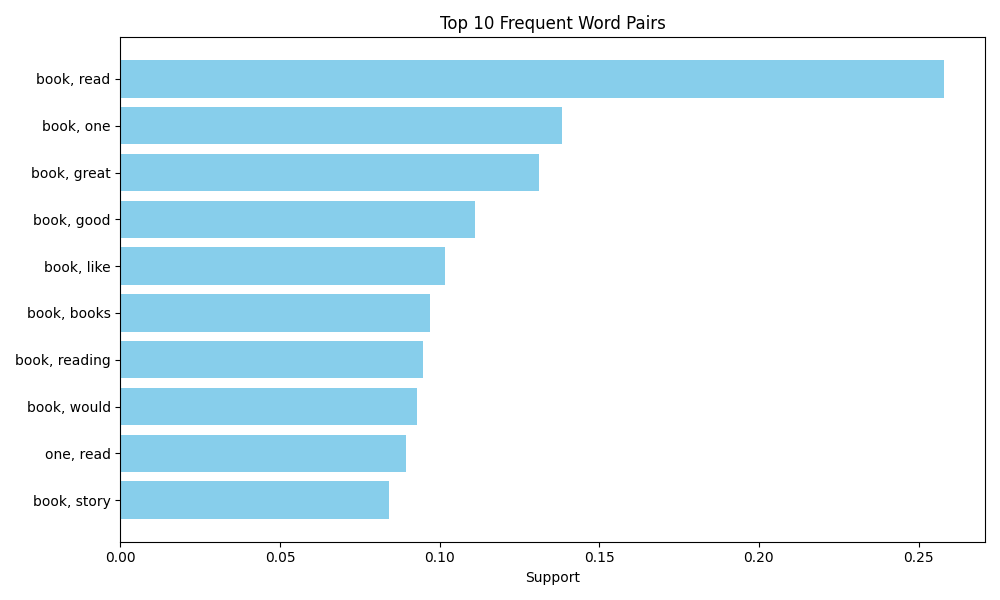
\includegraphics[width=0.8\textwidth]{../images/frequent_word_pairs.png}
\end{center}

\subsection*{Top Frequent Book Pairs}
\begin{center}
    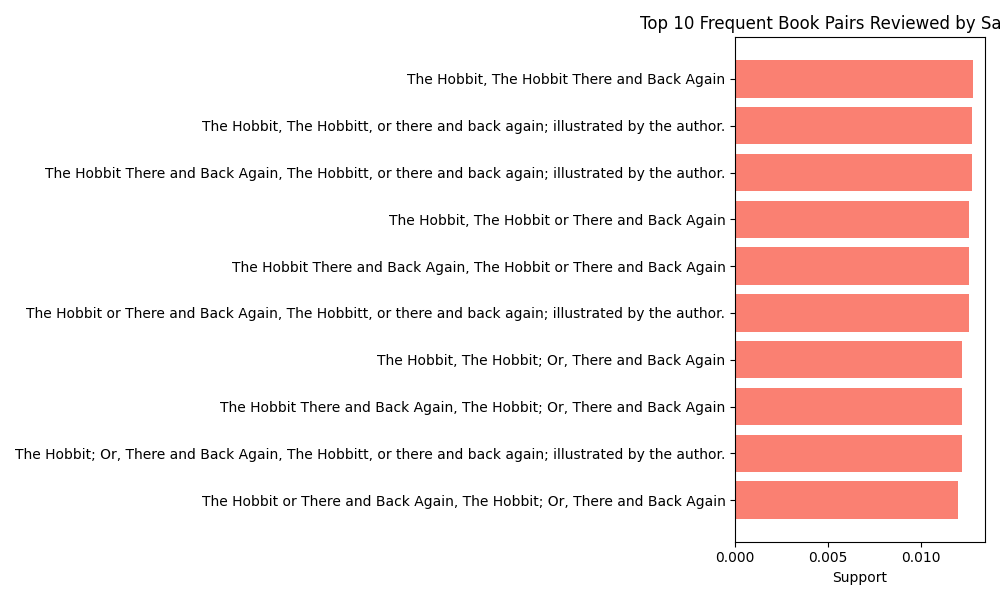
\includegraphics[width=0.8\textwidth]{../images/frequent_book_pairs.png}
\end{center}

\section{Scalability}
To ensure scalability:
\begin{itemize}
    \item We used \texttt{mlxtend}, which is optimized for large binary datasets.
    \item Used subsampling (1\%) during development to avoid Colab memory crashes.
    \item The approach is easily scalable by adjusting the sampling rate or chunking the dataset.
\end{itemize}

\section{Reflection}
\begin{itemize}
    \item Word baskets often cluster around sentiment or themes (e.g., “book, read”, “book, great”).
    \item Book baskets reveal user reading patterns, showing strong clustering around popular titles.
\end{itemize}

\section*{Declaration}
\textit{
I/We declare that this material, which I/We now submit for assessment, is entirely my/our own work and has not been taken from the work of others, save and to the extent that such work has been cited and acknowledged within the text of my/our work, and including any code produced using generative AI systems. I/We understand that plagiarism, collusion, and copying are grave and serious offences in the university and accept the penalties that would be imposed should I engage in plagiarism, collusion or copying. This assignment, or any part of it, has not been previously submitted by me/us or any other person for assessment on this or any other course of study.
}

\end{document}

